\documentclass[11pt]{book}
 
\newcommand{\reporttitle}{Coupling / Curtains}
\newcommand{\reportauthor}{CARIOU KOTLAREK}
\newcommand{\course}{Semester Paper}
\newcommand{\professor}{JACQUIER ; ACCIAIO}
% include file with configuration.
\input{../config/config_article} % various packages needed for maths etc.



\begin{document}


\begin{figure}[h]
\centering
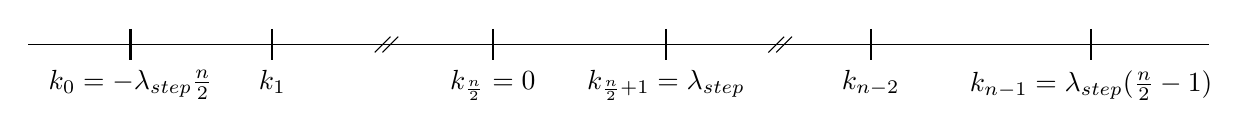
\begin{tikzpicture}
\foreach \x/\y in {
-6.2/ k_{0} = - \lambda_{step} \frac { n } { 2 } , 
-4.4/ k_{1},
0.6/ k_{ \frac{n}{2} + 1} = \lambda_{step} , 
-1.6/ k_{ \frac{n}{2}} = 0, 
3.2/ k_{n - 2}, 
6/ k_{n-1} =   \lambda_{step} (\frac { n } { 2 } - 1 )      }
 \draw[thick] (\x,0.2) -- (\x,-0.2) node[below]{$\y$};
\draw[thin] (-3,-0.10)--(-2.8 ,0.10);
\draw[thin] (-3.1,-0.10)--(-2.9 ,0.10);
\draw[thin] (1.9,-0.10)--(2.1 ,0.10);
\draw[thin] (2,-0.10)--(2.2 ,0.10);
\draw[thin] (-7.5,0)--(7.5 ,0);
\end{tikzpicture}
\end{figure}




\end{document}